\section{Problem statement}
\label{sec:problem}

While the integration of BCIs and continuous \gls{EEG} monitoring within serious games presents a promising avenue for neurocognitive assessment, translating these concepts into functional clinical tools requires a highly robust underlying hardware architecture \cite{craik2023design}. Fundamentally, the physical acquisition of this neural data begins with an \gls{EEG} cap fitted with non-invasive sensors designed to detect microvolt-level electrical signals from the cerebral cortex. Because these raw biological signals are inherently weak and highly susceptible to noise, they must be routed to a dedicated acquisition board or a multi-stage card system \cite{armand2024low}. This hardware typically consists of an analog front-end—responsible for the high-precision amplification, filtering, and digitization of the signals—and a digital processing unit, such as a microcontroller, for real-time data management and routing \cite{janapati2023advances}. To effectively map the neurocognitive responses elicited by the serious games, this continuous neural data must be contextually locked to specific in-game cognitive stimuli. This vital synchronization is achieved by interfacing the acquisition hardware with the stimulus presentation device, which transmits discrete event markers that map external gameplay milestones directly to the \gls{EEG} stream \cite{minissi2025role}.

However, the translation of this theoretical promise into clinical reality faces formidable engineering barriers. The efficacy of closed-loop interventions is predicated not on the mere availability of data, but on the fidelity and temporal determinism of that data \cite{sabio2024scoping}. Current acquisition architectures, particularly those designed for portability and low cost, are frequently plagued by systemic failures that sever the causal link between neural intention and digital response \cite{ariza2022low}. This research defines and analyzes two such sequential, critical failures. The foundational challenge stems from severe Signal-to-Noise Ratio (\gls{SNR}) limitations inherent to embedded architectures \cite{li2025high}. In portable \gls{EEG} devices designed for \gls{ADHD} monitoring, the physical proximity of high-speed digital processing components inevitably introduces electromagnetic interference. This interference degrades the system's high-precision analog sensing, corrupting the delicate microvolt-level neural signals required before any valid clinical evaluation can even begin \cite{dobrev2022high}. Once a reliable physiological signal is secured, a second, equally critical failure emerges: the precise synchronization of biomarkers \cite{esteban2026synchronization}. Because \gls{ADHD} neurocognitive assessments rely heavily on time-locked neural responses to specific game events, any temporal variability or unpredictable latency between the digital stimuli and the recorded biological signals fundamentally compromises the diagnostic validity of the data \cite{kaminski2026complexity}. The contrast between the theoretical promise of continuous monitoring and the clinical reality is summarized in Figure \ref{fig:general_barriers}.


\begin{figure}[h]
    \centering
    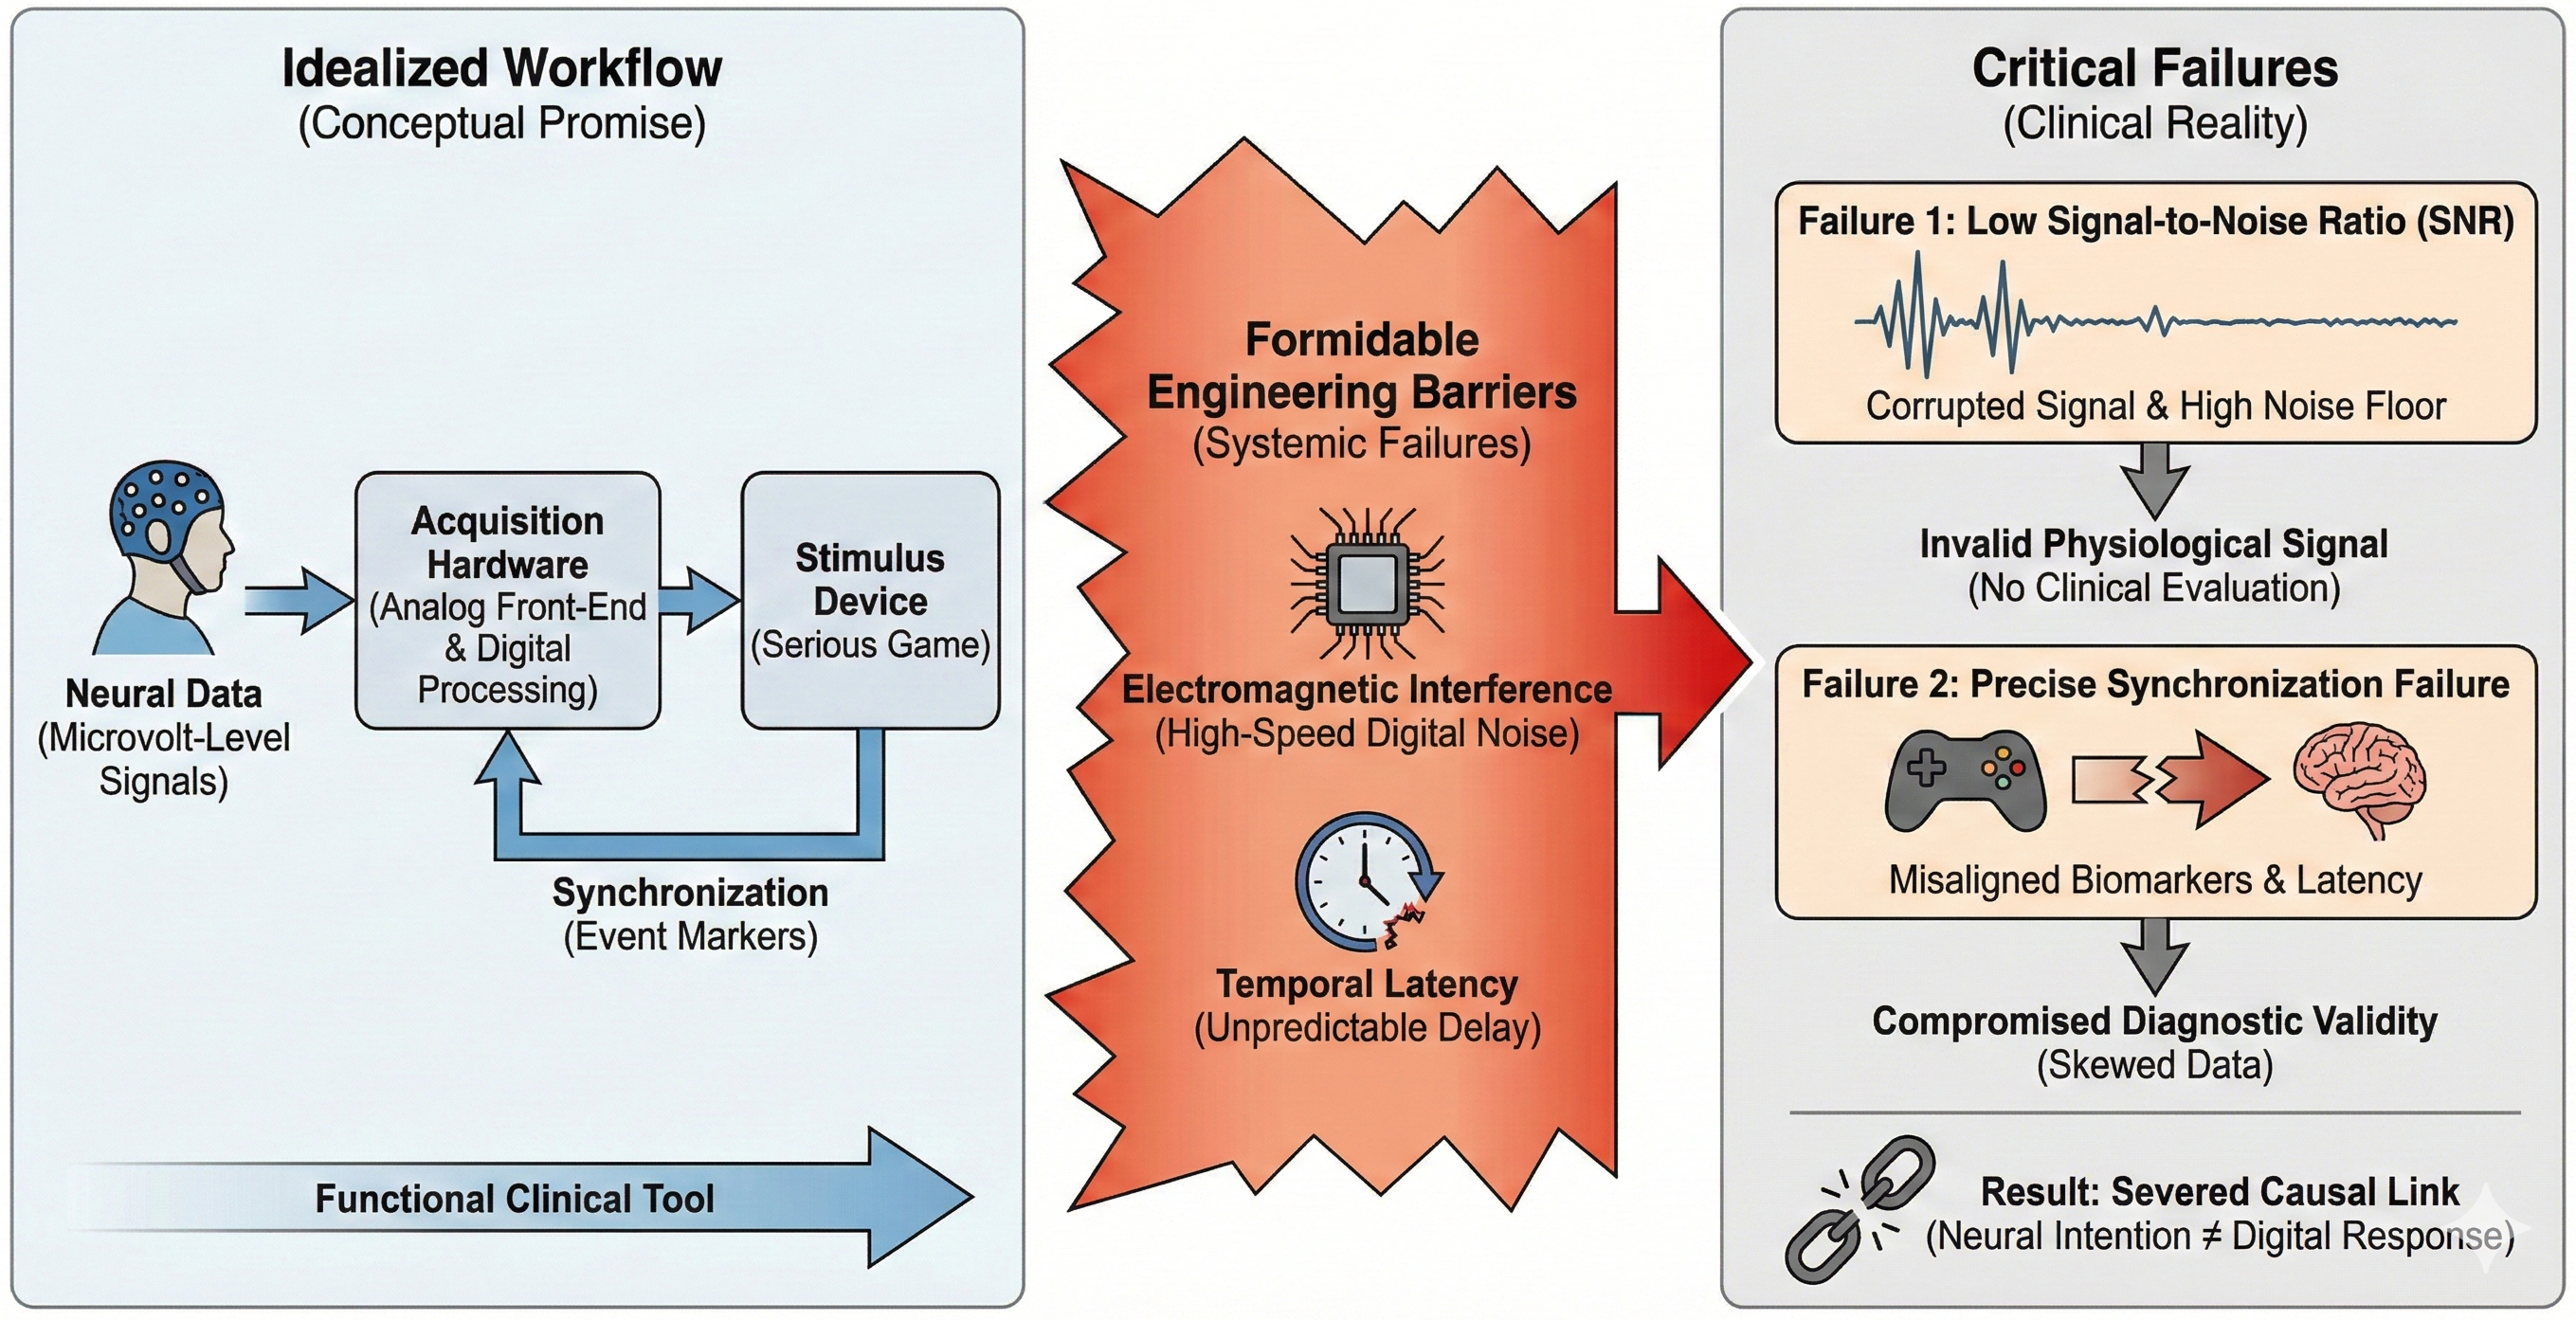
\includegraphics[width=0.8\linewidth]{Cap_1/Figures/Problem_general.png}
    \caption{The clinical translation problem in neurocognitive assessment systems. The illustration defines the two sequential critical failures that compromise diagnostic validity: the corruption of the analog signal and the temporal misalignment of biomarkers.}
    \label{fig:general_barriers}
\end{figure}


\subsection{SNR limitations in embedded systems}


The physical interface of traditional clinical EEG setups creates a major operational bottleneck for pediatric neurocognitive assessment. Lengthy and restrictive cap placement processes consistently induce restlessness, anxiety, and movement artifacts in children with ADHD \cite{Lim2023}. If the acquisition hardware cannot be deployed rapidly and comfortably, the resulting setup latencies and prolonged impedance stabilization times severely degrade the \gls{SNR} \cite{gorjan2022removal}. This physical friction directly compromises the ecological validity and engagement required for a serious game environment, making the rapid deployment of the acquisition cap a critical challenge to overcome \cite{kaongoen2023future}.

Once the physical interface is established, preserving analog signal integrity within a densely populated, mixed-signal embedded system presents a fundamental hardware challenge \cite{liu2024design}. The close physical proximity of high-speed digital processing units to the analog front-end introduces severe risks of electromagnetic interference and power supply noise coupling \cite{devi2022survey}. If physical board layout and isolation strategies are inadequate, the system's intrinsic background noise will inevitably exceed the baseline input-referred noise thresholds of the acquisition components (typically 1 µVpp) \cite{rashid2018eeg}. Overcoming this mixed-signal noise ceiling is essential; failure to do so creates a high noise floor that completely masks the low-amplitude Event-Related Potentials (\glspl{ERP}) necessary for cognitive assessment \cite{kim2022miniaturization}.

Even if analog noise is successfully mitigated, the embedded system's processing hardware faces severe resource constraints when managing continuous, high-frequency electrophysiological data streams. Unoptimized continuous data logging demands substantial computational power and can rapidly induce I/O bottlenecks, RAM saturation, and subsequent thermal throttling \cite{battaglia2022eeg}. The immediate consequence of an overburdened CPU or saturated memory footprint is the dropping of crucial data packets and the introduction of variable acquisition latency \cite{arroba2024sustainable}. This resource exhaustion fundamentally corrupts the integrity and continuity of the EEG data stream itself. Therefore, continuous monitoring of RAM usage and CPU load is critical to ensure the hardware can sustain reliable, uninterrupted data acquisition without buckling under the operational demands \cite{ajmeria2022critical}. As illustrated in Figure \ref{fig:hardware_bottlenecks}, the physical friction of traditional cap placement and the subsequent risk of analog signal corruption present immediate hurdles.


\begin{figure}[h]
    \centering
    \includegraphics[width=0.8\linewidth]{Cap_1/Figures/subproblem1.png}
    \caption{Physical, electrical, and computational resource barriers in deploying \gls{EEG} systems. The illustration highlights operational bottlenecks during patient setup, the risk of \gls{SNR} degradation due to mixed-signal interference, and embedded system resource exhaustion.}
    \label{fig:hardware_bottlenecks}
\end{figure}

\subsection{Synchronization and temporal variability in \gls{EEG} biomarkers}

The primary challenge in extracting valid neurocognitive assessments lies in the precise temporal synchronization of acquired \gls{EEG} biomarkers with external serious game stimuli \cite{ahmed2025eeg}. During interactive sessions, event markers are continuously transmitted from the game interface to the acquisition system. Standard communication protocols, however, introduce inherent, non-deterministic latency driven by transmission overhead, variable polling rates, and operating system scheduling conflicts \cite{buraimoh2023overview}. This unpredictable communication jitter fundamentally skews the temporal alignment between the stimulus presented to the patient and the corresponding neurophysiological response \cite{larsen2024method}. By conducting rigorous short-term latency bounding tests, this immediate communication delay must be quantified and mitigated to ensure the calculated Event-Related Potentials (ERPs) are temporally accurate and clinically viable \cite{he2023diversity}.

Beyond the immediate delay of single events, maintaining precise synchronization throughout a complete clinical session presents a compounding temporal challenge. Standard pediatric ADHD evaluations demand sustained, uninterrupted engagement. Continuous execution over these extended periods exposes the acquisition architecture to cumulative temporal errors \cite{arpaia2025acquisition}. Asynchronous clock drift between the event triggers and the hardware sampling rate, coupled with potential memory buffer saturation and thermal-induced performance fluctuations, introduces progressive instability \cite{dasenbrock2022synchronization}. This compounding jitter degrades deterministic data throughput, leading to a critical flaw where an ERP captured at the end of a session exhibits a fundamentally different latency profile than one captured at the beginning. Extended stability testing over full-length sessions is therefore imperative to prevent temporal degradation and validate the long-term reliability of the continuous EEG stream \cite{tran2026inter}.

In parallel with resolving these mechanical timing issues, valid synchronization relies on the system's proven ability to capture authentic, dynamic electrophysiological phenomena rather than structured noise \cite{correia2024brain}. Before complex ERPs can be reliably synchronized with external events, a foundational physiological baseline test must be conducted. This problem is addressed by detecting spontaneous frequency modulations, specifically the well-documented attenuation of alpha-band activity (8–13 Hz) when a subject transitions from an eyes-closed to an eyes-open state \cite{isler2023longitudinal}. If the signal processing pipeline distorts the bandwidth or lacks the sensitivity to capture these baseline spectral shifts, the recorded data is physiologically invalid \cite{flo2022automated}. Verifying the fundamental ability to resolve these basic frequency changes ensures that the synchronized event markers are anchored to genuine neural activity \cite{frelih2025modulation}. Figure \ref{fig:sync_challenges} demonstrates how non-deterministic latency and cumulative temporal drift fundamentally skew the alignment between the game stimulus and the neurophysiological response.

Finally, the temporal precision of the biomarkers must be matched by their spatial and structural integrity, which requires addressing inherent hardware vulnerabilities. High-resolution, multi-channel EEG acquisition creates a strict physical requirement for trace isolation to prevent analog signal bleed. Without meticulous shielding, adjacent channels inevitably suffer from crosstalk, blending distinct spatial brain waves and destroying the topographical accuracy of the recorded data. Furthermore, rendering these continuous data streams can introduce visualization artifacts that masquerade as genuine visual transients or \glspl{ERP}. By executing rigorous signal isolation and artifact detection tests, these structural issues can be identified and eliminated, ensuring that the precisely synchronized neurocognitive markers are extracted from pristine, uncontaminated data.



\begin{figure}[h]
    \centering
    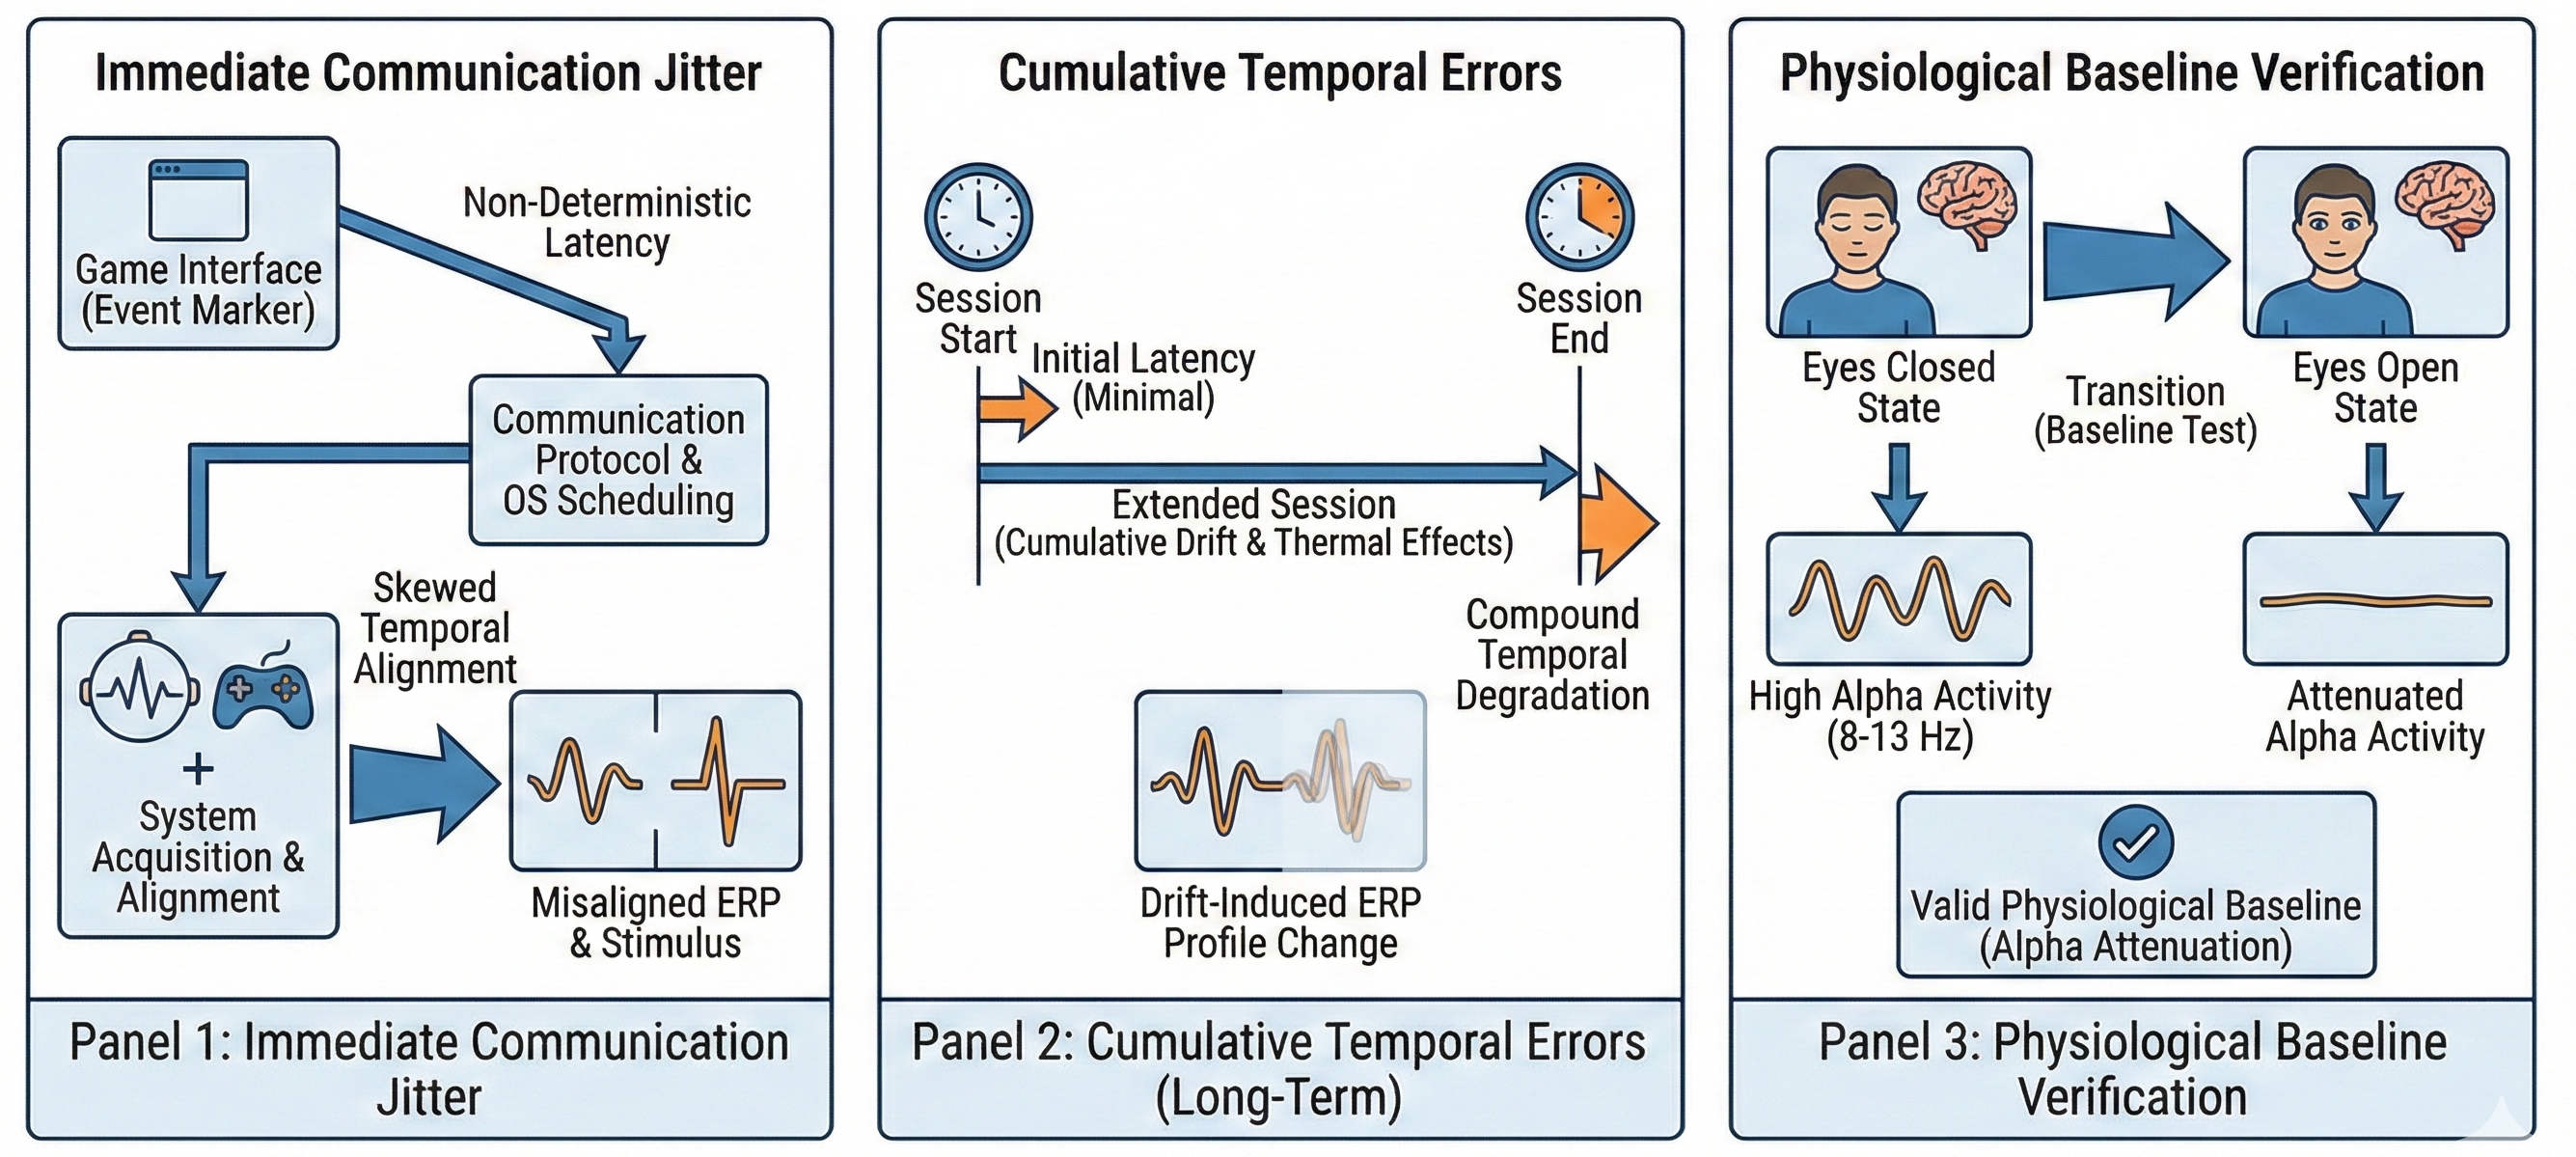
\includegraphics[width=0.8\linewidth]{Cap_1/Figures/subproblem2.png}
    \caption{Synchronization errors and real-time physiological validation. This figure details the impact of short-term non-deterministic communication jitter, cumulative temporal drift in extended sessions, and physiological baseline verification via alpha-band attenuation.}
    \label{fig:sync_challenges}
\end{figure}





\newpage
\section{Research question}\label{sec:question}

How can an embedded EEG acquisition architecture be optimized to simultaneously mitigate mixed-signal interference and non-deterministic synchronization jitter to ensure the clinical validity of biomarkers in serious-game-based ADHD assessments?


